\chapter* {Appendix}
\pagenumbering{gobble} % Appendix pages are not numbered




\section*{Github Actions}

\subsection*{Latex Compilation}
\begin{lstlisting}
name: Latex Compilation

# Only trigger, when the build workflow succeeded
on:
  push:
    paths:
      - 'Latex/**'
      - '.github/workflows/LatexCompilation.yml'

jobs:
  build_latex:
    runs-on: ubuntu-latest
    steps:
      - name: Set up Git repository
        uses: actions/checkout@v3
        
      - name: Compile LaTeX document
        uses: xu-cheng/latex-action@v2
        with:
          root_file: main.tex
          working_directory: ./Latex
          
      - name: Upload PDF file
        uses: actions/upload-artifact@v3
        with:
          name: PDF
          path: ./Latex/main.pdf
\end{lstlisting}

\subsection*{Python Tests}
\begin{lstlisting}
# This workflow will install Python dependencies, run tests and lint with a variety of Python versions
# For more information see: https://docs.github.com/en/actions/automating-builds-and-tests/building-and-testing-python

name: Python Tests

on:
  push:
    branches:
      - main
    paths:
      - 'Python_BNumMet/src/**'
      - 'Python_BNumMet/Demos/**'
      - 'Python_BNumMet/tests/**'
      - '.github/workflows/PythonTests.yml'
      - 'Python_BNumMet/requirements.txt'
      - 'Python_BNumMet/setup.py'
      - 'Python_BNumMet/pyproject.toml'
      - 'Python_BNumMet/setup.cfg'
      - 'Python_BNumMet/tox.ini'

jobs:
  test:
    runs-on: ${{ matrix.os }}
    strategy:
      matrix:
        os: [ubuntu-latest] #[ubuntu-latest, windows-latest, macos-latest]
        python-version: ['3.8', '3.11'] #['3.8', '3.9', '3.10', '3.11']

    steps:
    - uses: actions/checkout@v3
    - name: Set up Python ${{ matrix.python-version }}
      uses: actions/setup-python@v3
      with:
        python-version: ${{ matrix.python-version }}

    - name: Install dependencies
      run: |
        cd "Python_BNumMet"
        # Upgrade pip
        python -m pip install --upgrade pip 

        # tox-gh-actions is a plugin for tox that makes it work with GitHub Actions
        pip install tox tox-gh-actions 

        # for linting
        pip install flake8 

        # Requirements
        pip install -r requirements.txt

    - name: Lint with flake8
      run: |
        cd "Python_BNumMet"

        # stop the build if there are Python syntax errors or undefined names
        flake8 . --count --select=E9,F63,F7,F82 --show-source --statistics

        # exit-zero treats all errors as warnings. The GitHub editor is 127 chars wide
        flake8 . --count --exit-zero --max-complexity=10 --max-line-length=127 --statistics

    - name: Test with pytest
      run: |
        cd "Python_BNumMet"
        # Run tests
        tox
\end{lstlisting}

\subsection*{Python Publish}
\begin{lstlisting}
# This workflow will upload a Python Package using Twine when a release is created
# For more information see: https://docs.github.com/en/actions/automating-builds-and-tests/building-and-testing-python#publishing-to-package-registries

# This workflow uses actions that are not certified by GitHub.
# They are provided by a third-party and are governed by
# separate terms of service, privacy policy, and support
# documentation. 

name: Upload Python Package

on:
  workflow_run:
    workflows: ["Python Tests"]
    types:
      - completed # Only run, when the tests workflow Python Tests is completed
  push:
    branches:
      - main
    paths:
      - 'Python_BNumMet/VERSION' # Only trigger, when the version file is changed 
    


permissions: # https://docs.github.com/en/actions/reference/authentication-in-a-workflow#permissions-for-the-github_token
  contents: read

jobs:
  deploy: # https://packaging.python.org/guides/publishing-package-distribution-releases-using-github-actions-ci-cd-workflows/
    runs-on: ubuntu-latest
    if: ${{ github.event.workflow_run.conclusion == 'success' }} # Only run, if the tests succeeded 

    steps:
    - uses: actions/checkout@v3
    - name: Set up Python
      uses: actions/setup-python@v3
      with:
        python-version: '3.x'
    - name: Install dependencies
      run: |
        cd "Python_BNumMet"
        python -m pip install --upgrade pip
        pip install build
    - name: Build package
      run: |
        cd "Python_BNumMet" 
        python -m build
    - name: Publish package
      uses: pypa/gh-action-pypi-publish@release/v1
      with:
        user: __token__
        password: ${{ secrets.PYPI_TOKEN }}
        packages-dir: Python_BNumMet/dist/
\end{lstlisting}


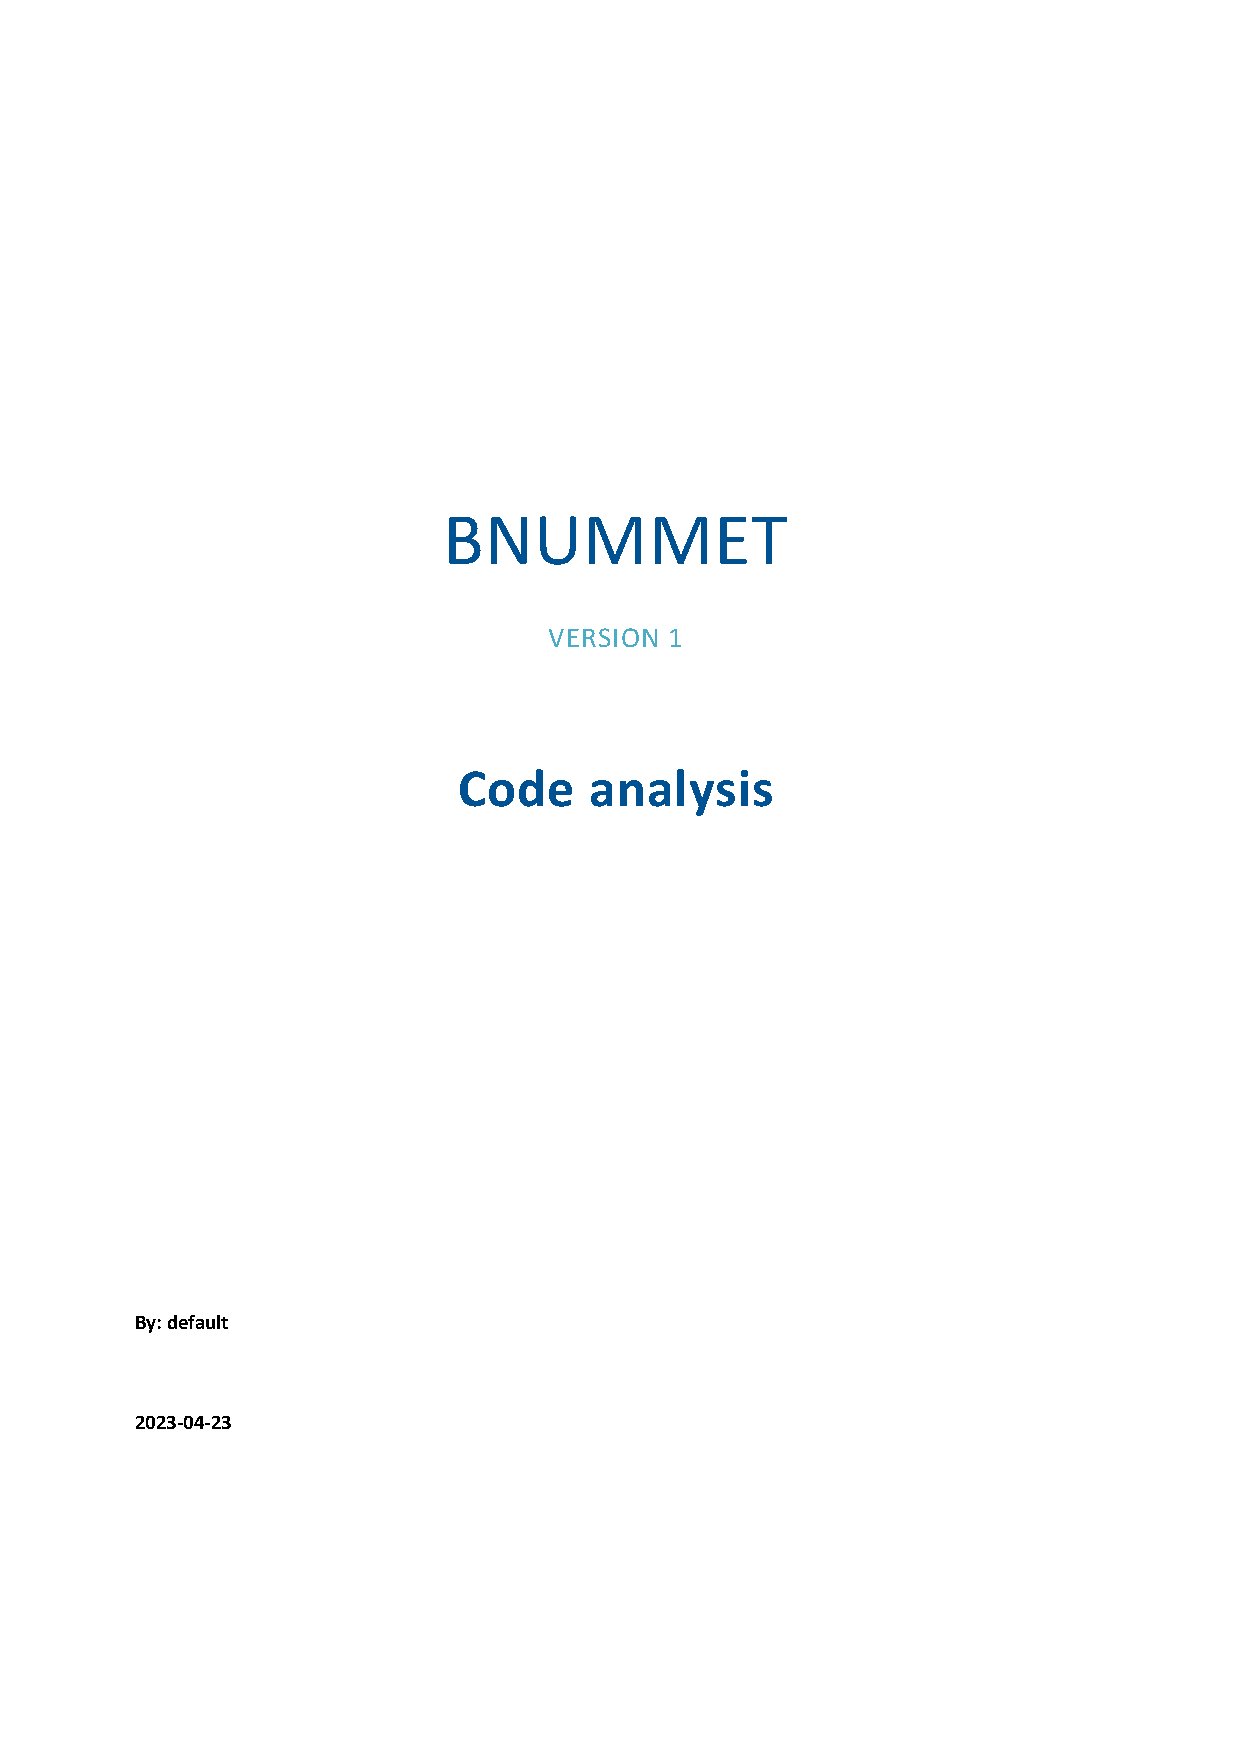
\includepdf[pages=1,scale=1,pagecommand=\section*{SonarQube Report}]{Include/PDFs/BNumMet-analysis-report.pdf}
\includepdf[pages=2-,scale=1]{Include/PDFs/BNumMet-analysis-report.pdf}